% Editable vector copy of MBE-drawing.svg (whose labels were flattened to paths).
% Commutative diagram of the KG kinematics for a thin-walled arterial ring,
% with notation consistent with the manuscript (F = F_e F_g, roman subscripts).
% Compile:  pdflatex mbe-scheme.tex   ->  mbe-scheme.pdf
\documentclass[border=8pt]{standalone}
\usepackage{amsmath,amssymb}
\usepackage{tikz}
\usetikzlibrary{arrows.meta,calc}

% ---- a thin-walled ring; #1 centre, #2 outer r, #3 inner r, #4=1 adds pressure
\newcommand{\ring}[4]{%
  \begin{scope}
    \fill[gray!55,even odd rule] (#1) circle (#2) (#1) circle (#3);
    \draw[line width=0.4pt] (#1) circle (#2);
    \draw[line width=0.4pt] (#1) circle (#3);
    \fill (#1) circle (1.1pt);
    \ifnum#4=1
      \foreach \a in {0,45,...,315}{%
        \draw[blue,-{Latex[length=1.6mm]}] ($(#1)+(\a:0.50*#3)$)--($(#1)+(\a:0.85*#3)$);}
    \fi
  \end{scope}}

% ---- wall-thickness dimension: two arrows pointing toward each other across the
%      wall (tips at inner and outer surface, gap = thickness). #1 c #2 rout #3 rin #4 angle
\newcommand{\thickdim}[4]{%
  \draw[-{Latex[length=2.0mm]},line width=0.7pt] ($(#1)+(#4:#2+0.34)$)--($(#1)+(#4:#2)$);
  \draw[-{Latex[length=2.0mm]},line width=0.7pt] ($(#1)+(#4:#3-0.34)$)--($(#1)+(#4:#3)$);}

\begin{document}
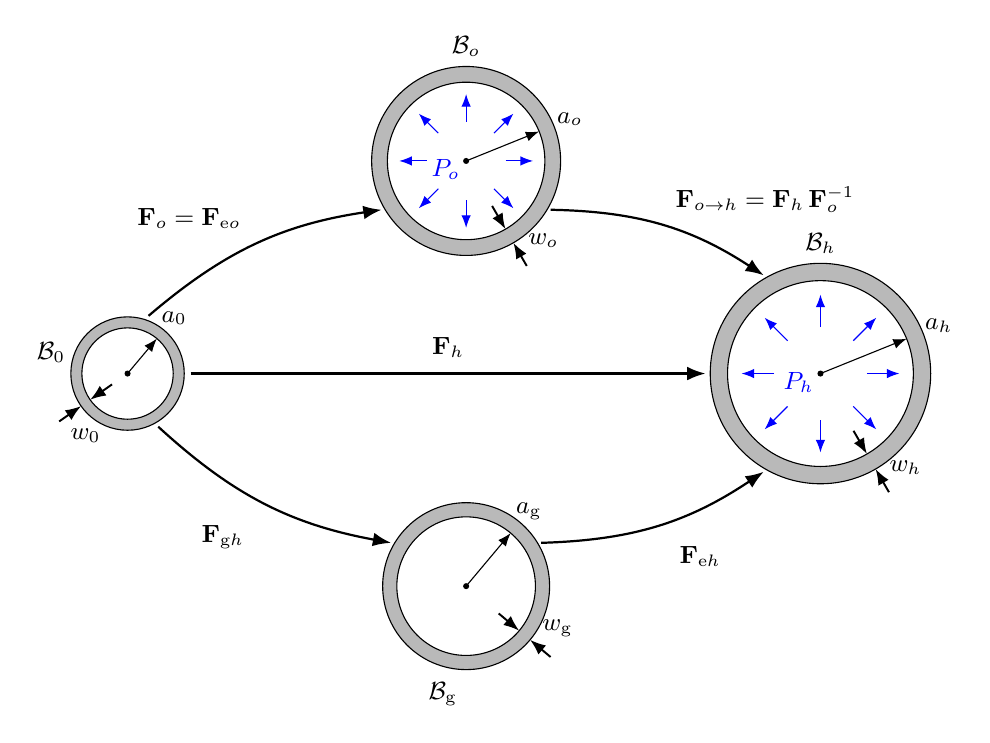
\begin{tikzpicture}[>=Latex,font=\small,line join=round]

  \coordinate (C0) at (0,0);        % reference        B_0
  \coordinate (Co) at (4.3,2.7);    % original homeo   B_o (pressurised)
  \coordinate (Cg) at (4.3,-2.7);   % grown natural    B_g
  \coordinate (Ch) at (8.8,0);      % evolved homeo    B_h (pressurised)

  % ---------- rings ----------
  \ring{C0}{0.72}{0.58}{0}         % reference (unloaded)
  \ring{Co}{1.20}{1.00}{1}         % original homeostatic (pressurised)
  \ring{Cg}{1.06}{0.88}{0}         % grown natural (unloaded)
  \ring{Ch}{1.40}{1.18}{1}         % evolved homeostatic (pressurised)

  % ---------- geometry labels (radius arrow -> inner wall, label OUTSIDE) --------
  % reference B_0
  \draw[->] (C0)--($(C0)+(50:0.58)$);
  \node at ($(C0)+(50:0.92)$){$a_{0}$};
  \thickdim{C0}{0.72}{0.58}{215}
  \node at ($(C0)+(215:0.89)+(305:0.34)$){$w_{0}$};
  \node[left] at ($(C0)+(158:0.72)$){$\mathcal{B}_{0}$};
  % original homeostatic B_o (radius in the 0--45 gap; p at centre in the 180--225 gap)
  \draw[->] (Co)--($(Co)+(22:1.00)$);
  \node at ($(Co)+(22:1.42)$){$a_{o}$};
  \thickdim{Co}{1.20}{1.00}{300}
  \node at ($(Co)+(300:1.37)+(30:0.34)$){$w_{o}$};
  \node[blue] at ($(Co)+(202:0.28)$){$P_{o}$};
  \node[above] at ($(Co)+(90:1.20)$){$\mathcal{B}_{o}$};
  % grown natural B_g
  \draw[->] (Cg)--($(Cg)+(50:0.88)$);
  \node at ($(Cg)+(50:1.24)$){$a_{\mathrm g}$};
  \thickdim{Cg}{1.06}{0.88}{320}
  \node at ($(Cg)+(320:1.23)+(50:0.34)$){$w_{\mathrm g}$};
  \node[below] at ($(Cg)+(255:1.14)$){$\mathcal{B}_{\mathrm g}$};
  % evolved homeostatic B_h
  \draw[->] (Ch)--($(Ch)+(22:1.18)$);
  \node at ($(Ch)+(22:1.62)$){$a_{h}$};
  \thickdim{Ch}{1.40}{1.18}{300}
  \node at ($(Ch)+(300:1.57)+(30:0.34)$){$w_{h}$};
  \node[blue] at ($(Ch)+(202:0.30)$){$P_{h}$};
  \node[above] at ($(Ch)+(90:1.40)$){$\mathcal{B}_{h}$};

  % ---------- deformation maps ----------
  % reference -> original homeostatic (pure elastic; carries deposition stretches)
  \draw[->,thick] ($(C0)+(70:0.78)$) to[bend left=16]
        node[pos=0.5,above left=2pt]{$\mathbf{F}_{o}=\mathbf{F}_{\mathrm{e}o}$}
        ($(Co)+(210:1.24)$);
  % reference -> evolved homeostatic (total)
  \draw[->,thick] ($(C0)+(0:0.80)$)--
        node[midway,above=2pt]{$\mathbf{F}_{h}$} ($(Ch)+(180:1.46)$);
  % reference -> grown natural (growth part); arrives B_g at 150 deg
  \draw[->,thick] ($(C0)+(-60:0.78)$) to[bend right=16]
        node[pos=0.5,below left=4pt]{$\mathbf{F}_{\mathrm{g}h}$}
        ($(Cg)+(150:1.10)$);
  % grown natural -> evolved homeostatic (elastic part); leaves B_g at 30 deg
  \draw[->,thick] ($(Cg)+(30:1.10)$) to[bend right=16]
        node[pos=0.5,below right=4pt]{$\mathbf{F}_{\mathrm{e}h}$}
        ($(Ch)+(240:1.44)$);
  % original homeostatic -> evolved homeostatic (relative deformation, correct order)
  \draw[->,thick] ($(Co)+(330:1.24)$) to[bend left=16]
        node[pos=0.5,above right=1pt]{$\mathbf{F}_{o\to h}=\mathbf{F}_{h}\,\mathbf{F}_{o}^{-1}$}
        ($(Ch)+(120:1.44)$);

\end{tikzpicture}
\end{document}
